\chapter{Core Knowledge}\label{cap:planificación}

\section{Introducción}

En la actualidad existen numerosas técnicas empleadas en inteligencia artificial. Estas no provienen solo de física o matemáticas, sino que también llegan a estar estrechamente relacionadas con economía e informática. Es tal el catálogo de posibilidades del que disponemos que en numerosas ocaciones resulta complicado permanecer actualizado, ya que cada día surgen ideas nuevas. Por ello, con el objetivo de obtener el mayor entendimiento general del presente trabajo, vamos a explicar los principios de algunos métodos o técnicas emepleados en el proyecto, ya que la comprensión de estos falicitará seguir el flujo de trabajo. 

De este modo, comenzaremos hablando sobre algunos de los pilares, como qué son las redes neuronales, para luego profundizar en conceptos clave, tales como funciones de activación concretas o métodos de interpretabilidad.


\section{Redes neuronales}

Si echamos un vistazo a la historia de la ciencia y la tecnología, observaremos que muchos avances se inspiran en sistemas biológicos reales. Por ejemplo, una cámara fotográfica comparte muchas similitudes con el ojo humano. Otro ejemplo es el procesador, que consiste en un gran número de transistores conectados para realizar cálculos. Las redes neuronales también forman parte de esta tendencia, ya que su estructura se basa aproximadamente en las redes neuronales biológicas. Por esta razón, introduciremos brevemente este concepto antes de hablar de las redes neuronales artificiales.

\subsection{Neuronas}

Biologicamente hablando, una neurona es la unidad más pequeña del sistema nervioso, se encarga de recibir, procesar y transmitir información mediante impulsos eléctricos. Tienen tres componentes principales:

\begin{itemize}
    \item El cuerpo celular o soma contiene el núcleo y los orgánulos necesarios para el correcto funcionamiento de la neurona. Todas las señales que recibe la neurona por medio de las dendritas son transmitida a esta sección. Si la suma de dichas señales superan un determinado umbral en el cono axónico,  se genera un nuevo impulso eléctrico como respuesta que será propagado por el axón. Esta zona es especializada en esta labor, gracias a su gran concentración de sodio. Al incrementar el número de conexiones entre neuronas estas se vuelven más rápidas, permitiéndonos pensar con mayor velocidad, es decir, las ciertas tareas nos llevan menos tiempo. Este proceso, donde una neruona transmite información a otra se conoce como sinapsis.
    \item Dendritas: Son extensiones provenientes del soma. Son las encargadas de transmitir los impulsos eléctricos transmitidos por otras neuronas hasta el soma.  
    \item El axón es una larga proyección que se extiende desde el soma -normalmente originado en el montículo axónico- hacia los terminales sinápticos. Su función principal es transmitir impulsos eléctricos desde el cuerpo celular a otras neuronas, músculos o glándulas.
    \item Los terminales sinápticos tienen muchas ramificaciones, cada una de las cuales termina en un botón sináptico. Estas estructuras son las encargadas de liberar la señal eléctrica hacia otras células.
\end{itemize}

\begin{figure}[h!]
    \centering
    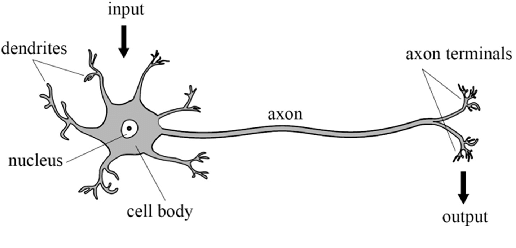
\includegraphics[width=0.6\textwidth]{figures/neural_parts.png}
    \caption{Parts of a neuron. Source: \cite{partsNeuron}}
    \label{fig:neuron}
\end{figure}

\subsection{Redes neuronales virtuales}

Comprender el origen de las redes neuronales puede ser crucial para mejorar nuestra metodología. Como ya sabemos qué es una red neuronal, a continuación presentaremos su homóloga virtual. Al hablar de las redes neuronales artificiales, las compararemos con sus equivalentes biológicas para profundizar en nuestra comprensión del tema. El objetivo es tomar conciencia de que las diferencias entre ellas no son tan significativas como puede parecer.

\subsubsection{Perceptron simple}


El perceptrón simple es uno de los modelos más básicos de red neuronal artificial. Funciona de forma similar a una neurona biológica. Recibe múltiples entradas, cada una de ellas multiplicada por un peso asociado, las suma y, a continuación, aplica una función de activación, normalmente una función umbral o sigmoidea. En el caso de la función umbral, si la suma ponderada de las entradas supera un determinado umbral, el perceptrón emite una señal (normalmente 1); en caso contrario, no (normalmente 0).
Dado que este proceso se asemeja al biológico, podemos pensar en él de la siguiente manera: la neurona recibe información (entradas), que se transmite hacia el núcleo, de forma análoga a la función de activación en las neuronas artificiales, y, si la señal es lo suficientemente fuerte, la neurona emite una nueva señal, similar a la salida de la función de activación.

\begin{figure}[h!]
    \centering
    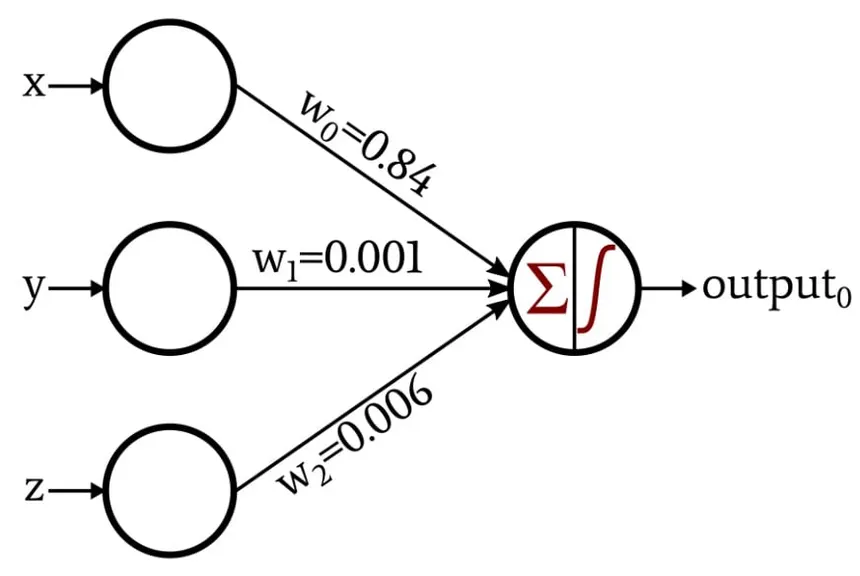
\includegraphics[width=0.6\textwidth]{figures/simple_perceptron.png}
    \caption{Simple perceptron. Source: \cite{simplePerceptron}}
    \label{fig:simplePerceptron}
\end{figure}

Una vez establecido el funcionamiento conceptual del perceptrón, conviene presentar su fundamento matemático. Analizar cómo el perceptrón transforma los datos en el espacio de entrada (normalmente un plano en dos dimensiones) puede aportar información valiosa para diseñar arquitecturas de redes neuronales más eficaces.

\section{Árboles de predicción}


\section{Valores Shap}